\section{Experimental Evaluation}
In this section, we report the initial findings of a benchmarking study we conducted. 
The goal of the benchmark study was to understand the relationship of the metric number of CPU cycles per probe input tuple ($C_{probe}$) with size of the probed hash table ($SizeHT$).

\begin{figure}[t]
	\centering
	\subfigure[Non Partitioned Probe]{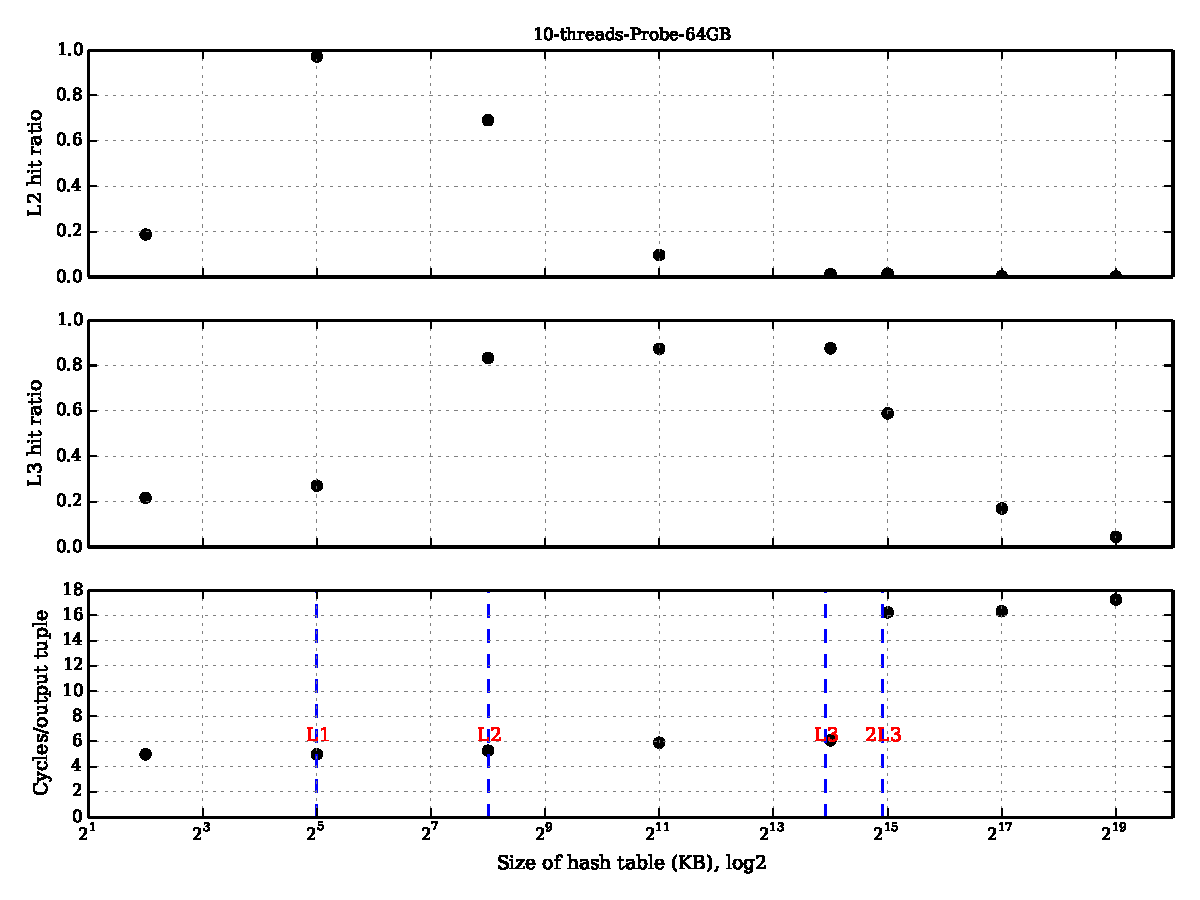
\includegraphics[width=0.5\textwidth]{figures/10-threads-Probe-64GB.pdf}}
	\subfigure[Partitioned Probe]{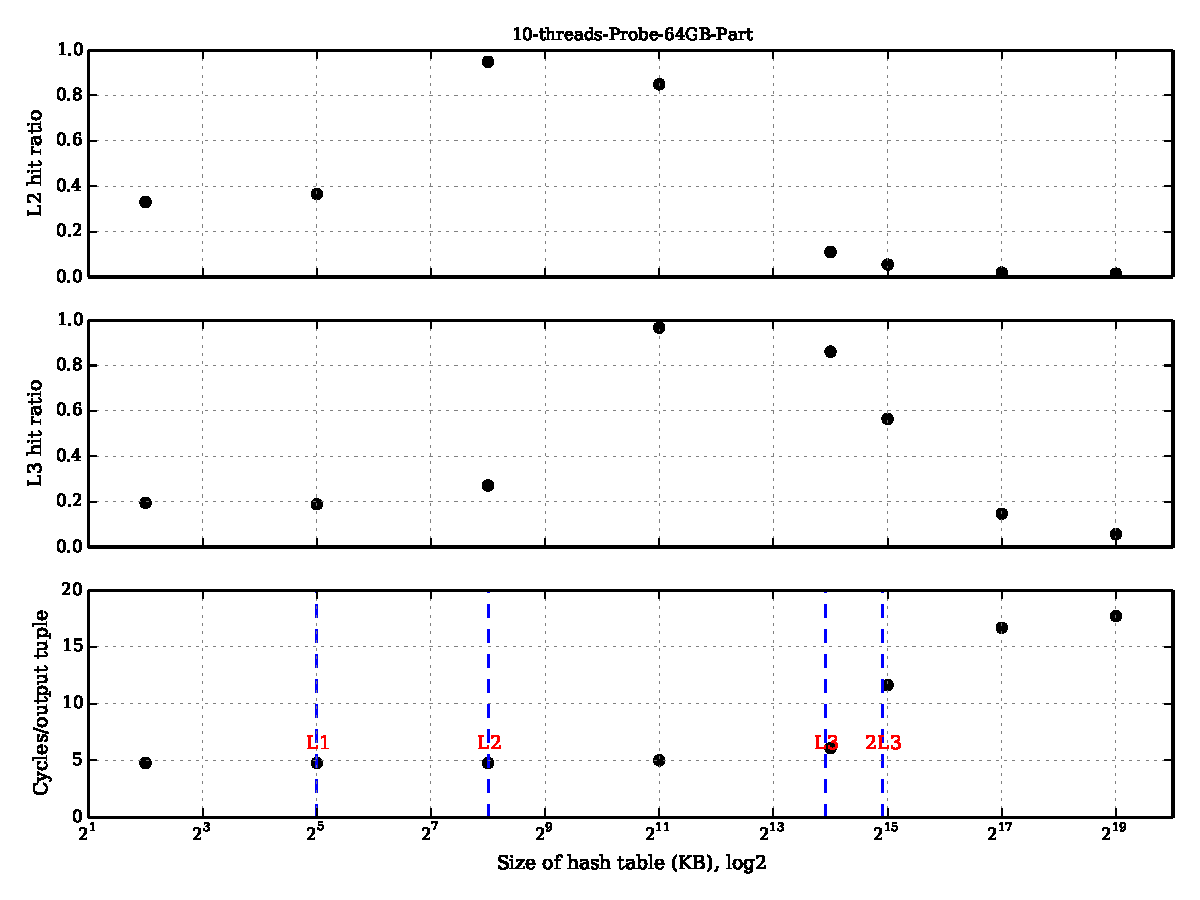
\includegraphics[width=0.5\textwidth]{figures/10-threads-Probe-64GB-Part.pdf}}
	\vspace{-0.6em}
	\caption{\textbf{Results for 10 threads and 64 GB probe input}}
	\label{fig:10threads-64gbprobe}
	\vspace{-1em}
\end{figure}

\reminder{Machine description.}

We developed a C++ prototype that mimics a probe operation. 
We implemented the probe operation in both partitioned and non-partitioned ways.
Note that the measurement does not include time to partition the probe table. 
We use Intel PCM for measuring the cache hit ratios and rdtsc counters for measuring the CPU cycles. 

Figure~\ref{fig:10threads-64gbprobe} presents the results from a probe operation using 10 threads and an input probe table of size 64 GB, and Figure~\ref{fig:10threads-32gbprobe} refers to the results of a probe operation that uses 10 threads and a 32 GB input probe table. 
On the X-axis is the size of hash table in KB (log scale). 
The three scatter plots indicate the CPU cycles per input tuple, L2 hit ratio and L3 hit ratio. 
To put the cache sizes in perspective, the blue dotted lines mark the sizes of L1, L2, and L3 caches. 
As the server machine has two NUMA sockets, we also added another line to mark 2*L3 size. 

Note the increase in CPU cycles per probe operation after the hash table sizes greater than L3. 

\begin{figure}[t]
	\centering
	\subfigure[Non Partitioned Probe]{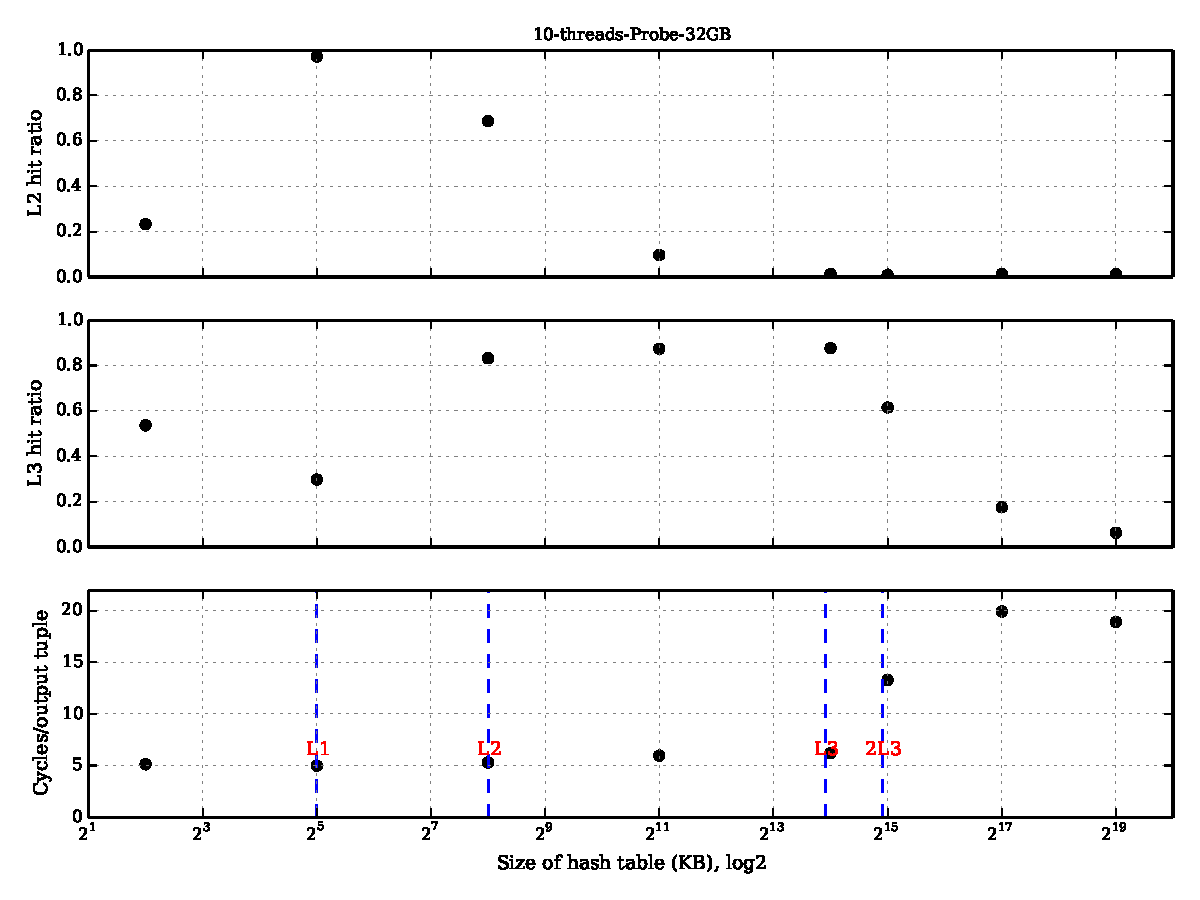
\includegraphics[width=0.5\textwidth]{figures/10-threads-Probe-32GB.pdf}}
	\subfigure[Partitioned Probe]{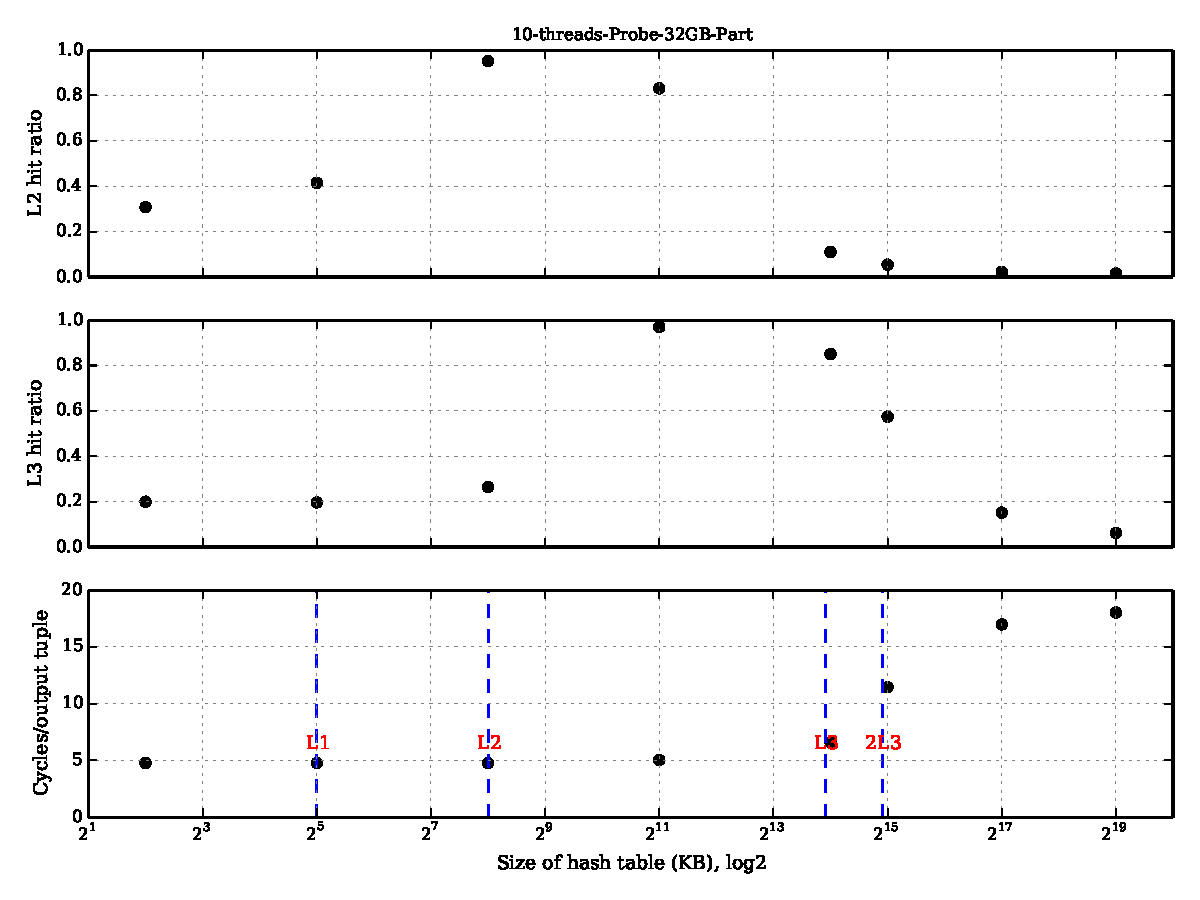
\includegraphics[width=0.5\textwidth]{figures/10-threads-Probe-32GB-Part.pdf}}
		\vspace{-0.6em}
	\caption{\textbf{Results for 10 threads and 32 GB probe input}}
	\label{fig:10threads-32gbprobe}
		\vspace{-1em}
\end{figure}

Note that the experiments using 10 threads don't make use of hyper threading. 
We perform the same experiment using all 20 threads on a single socket, which also includes the hyper-threading contexts. 
Figure~\ref{fig:20threads-32gbprobe} presents the results of this experiment. 
Notice that on sizes greater than 2*L3, the CPU cycles per input tuple is drastically higher (around 40) than that in the 20 threads case. 
However the impact of hyper threading is not as drastic for hash table sizes smaller than the size of the L3. cache 

\begin{figure}[t]
	\centering
	\subfigure[Non Partitioned Probe]{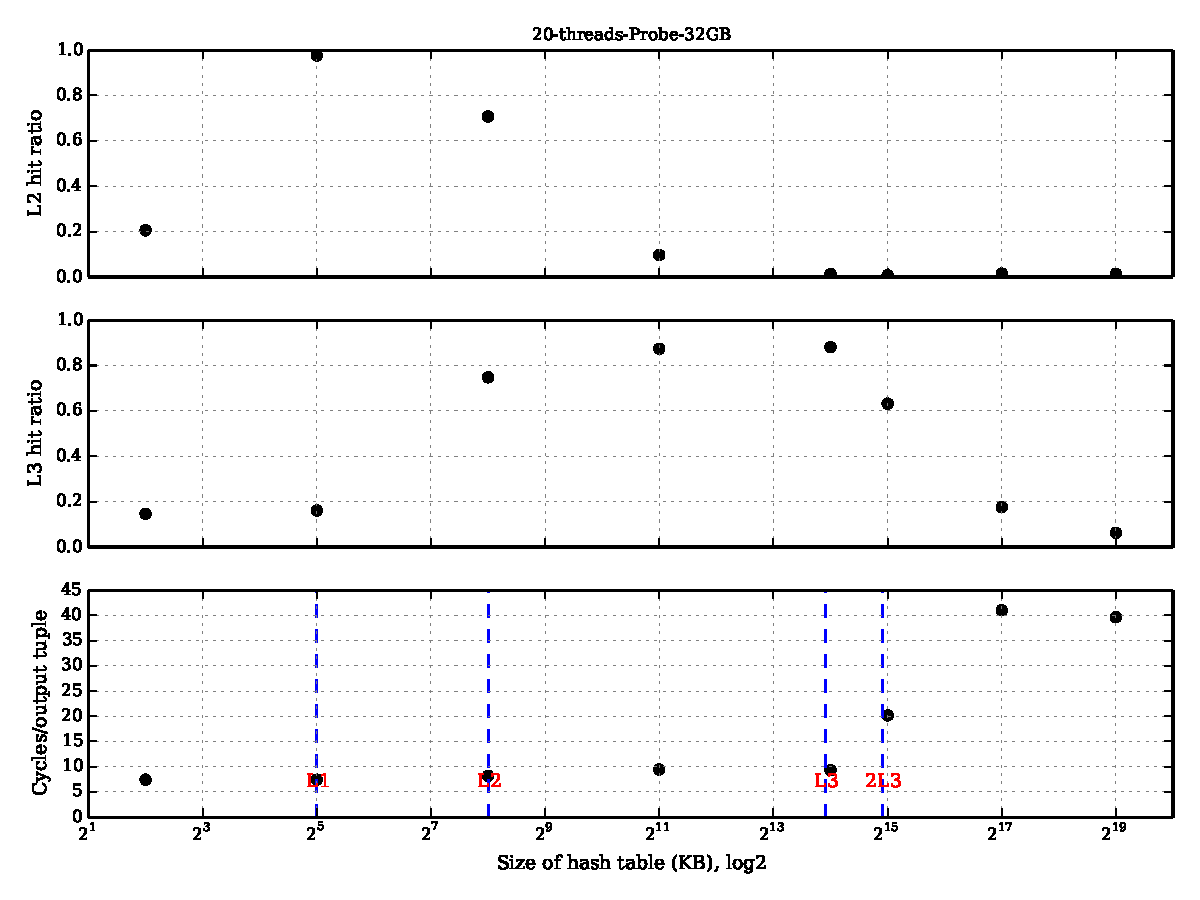
\includegraphics[width=0.5\textwidth]{figures/20-threads-Probe-32GB.pdf}}
	\subfigure[Partitioned Probe]{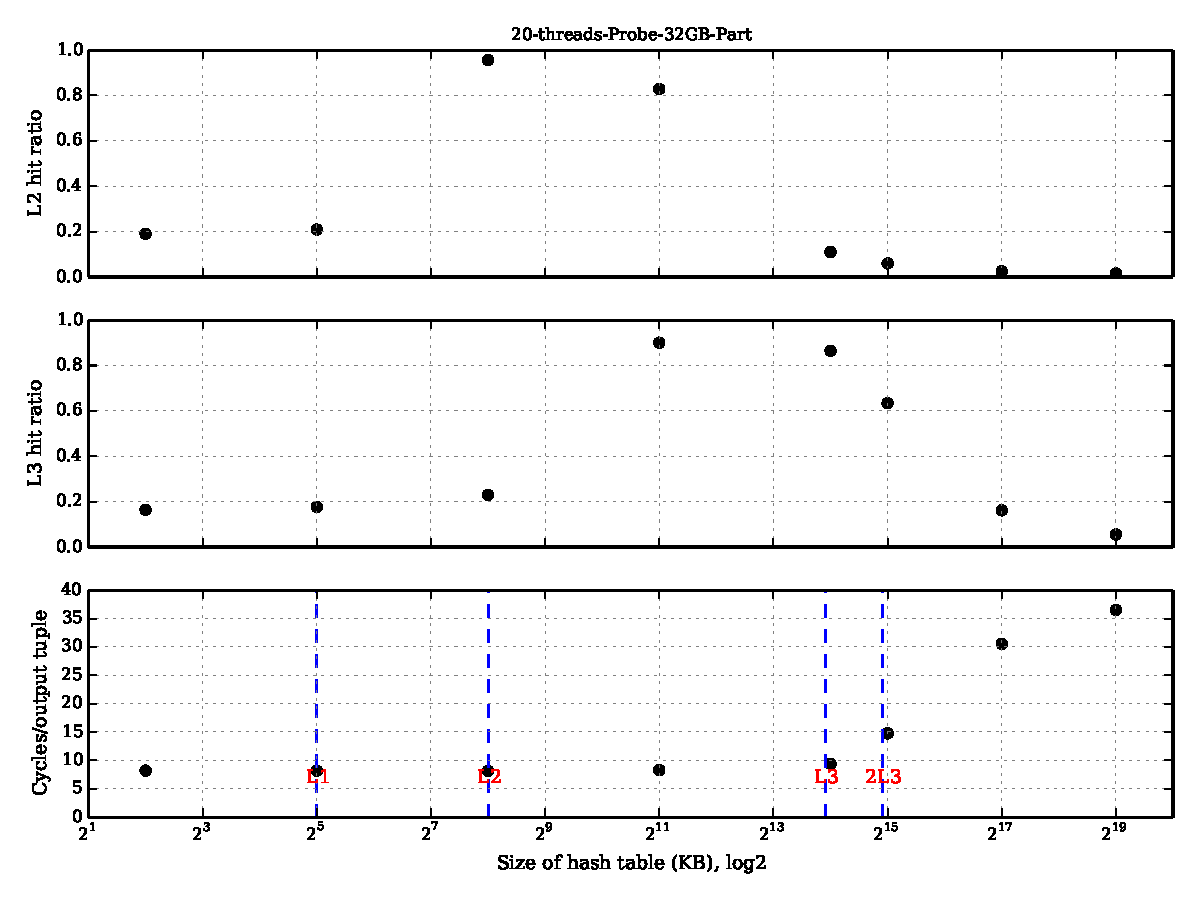
\includegraphics[width=0.5\textwidth]{figures/20-threads-Probe-32GB-Part.pdf}}
		\vspace{-0.6em}
	\caption{\textbf{Results for 20 threads and 32 GB probe input}}
	\label{fig:20threads-32gbprobe}
		\vspace{-1em}
\end{figure}